%\textcolor{red}{\hrulefill \textsc{Unfinished Section}\hrulefill}  \\
It is well known however that the standard model of particle physics cannot account for all observed phenomena.
Gravity, Dark Matter, and why the Higgs is so light, to name a few.
For this we often look to \emph{extend} the standard model to include more symmetries of nature.
These symmetries often include new fundamental particles that can be observed in experiments like ATLAS.
One such extension, \emph{Supersymmetry} (SUSY), is seen as potential Swiss army knife of answers to several unanswered problems in physics.
The idea here is that there is an explicit mathematical relationship, a symmetry, between fermions and bosons.
Whereas in the SM these two types of particles though very similar, are not treated on that same footing as they are in SUSY.
i.e. they really are two sides to the same coin in SUSY. 
Now the cool part is that when you introduce this symmetry you necessarily generate a doubling of all the fundamental particles described by the standard model.
Each fermion now has a bosonic mirror, a \emph{superpartner}, and equivalently each boson has a fermionic superpartner.
For what is called the Minimal Supersymmetric Standard Model (MSSM), whereby we have supersymmetry with the fewest number of particles added to the standard model the particle content can be seen in Figure~\ref{fig:theory:particlesSUSY} (post-EWK symmetry breaking).
Where we will also notice that in SUSY an additional $SU(2)$ Higgs doublet must be added\footnote{Due to the Higgs superfield (SUSY quantum fields) not being holomorphic an additional Higgs doublet must be added in order to cancel anomalies and be able the generate mass for both the up and down type quarks.}.
Supersymmetric fermions are called sfermions (squarks and sleptons) and supersymmetric gauge bosons are gauginos (Wino, Zino, gluino, Higgsino, and photino) and are all denoted with a the symbol of their standard partner with a tilde (\~X).
Now this is an experimental physicist's dream as there are now a whole bunch of potential new particles to discover, but of course that's not what we observe in nature, i.e. we would have seen (in abundance!) superpartners at the same masses as their 'standard' partners' masses.
This then means that the supersymmetry symmetry is broken.
Fortunately for us this symmetry can be broken in such a way that the particle masses are large and observable at collider experiments (with sufficient energy).
\begin{figure}[tbp]
  \begin{center}
    \includegraphics[width=0.98\textwidth]{figs/theory/SMtoSUSYparticleContent.png}
  \end{center}
  \caption[Particle content of the minimal supersymmetric standard model]{Particle content of the minimal supersymmetric standard model~\cite{KEK:2012}.}
  \label{fig:theory:particlesSUSY}
\end{figure}

We can now note how SUSY can address some of the unanswered questions in physics we listed in the beginning of this section.
One of which it can explicitly address is known as the Hierarchy Problem, or as I put it before, ``why is the Higgs so light.''
The problem can be stated as follows: if the standard model is valid all the way up to the Planck scale, would expect the mass of the Higgs, due to the perturbative loop corrections seen in Figure~\ref{fig:theory:HiggsMassLoops}, to be on the order of the Planck scale.
We of course do not see this with the observed mass of 125~\GeV of a SM like Higgs.
\begin{figure}[ht]
  \begin{center}
    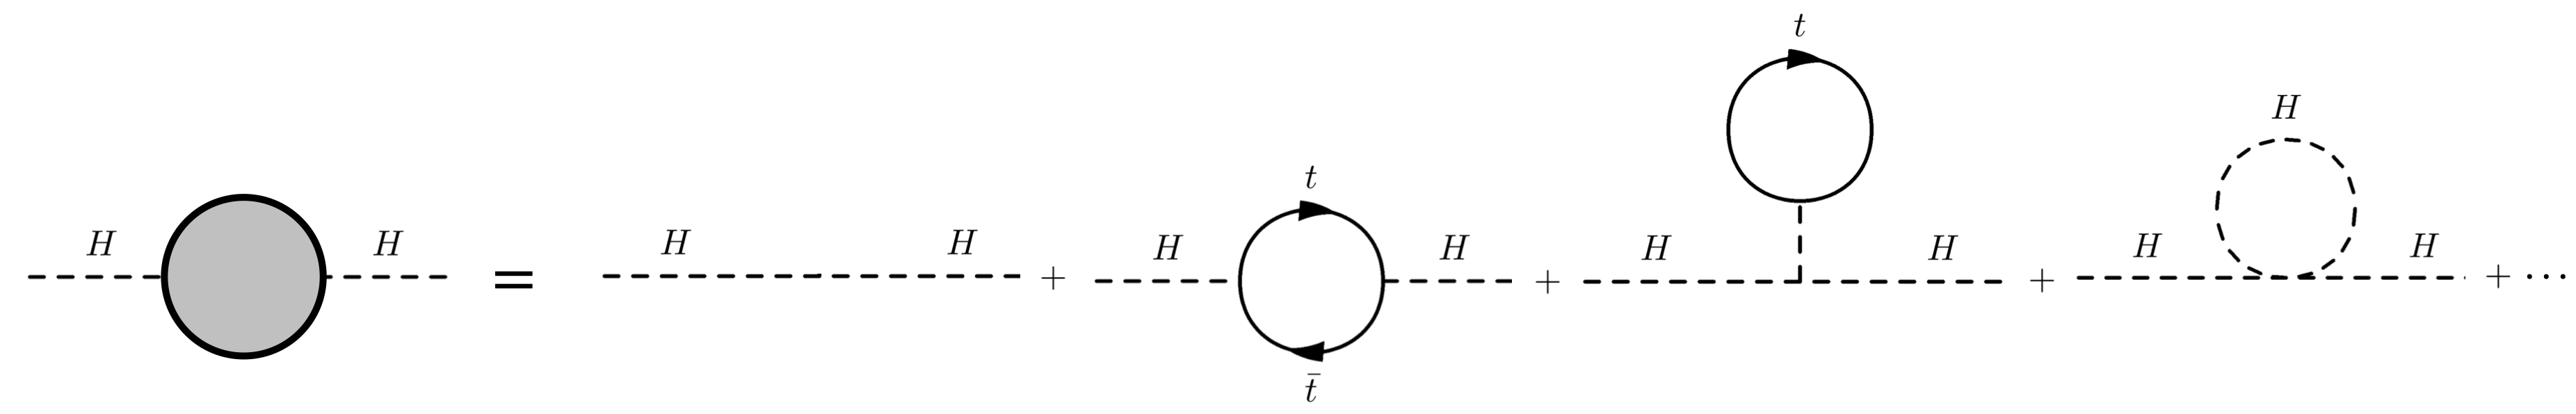
\includegraphics[width=0.98\textwidth]{figs/theory/HiigsMassLoops.png}
  \end{center}
  \caption{The observed Higgs mass as a sum of the bare Higgs mass plus loop corrections.}
  \label{fig:theory:HiggsMassLoops}
\end{figure}
With the addition of superparters we find that a delicate cancellation occurs, where large loop corrections to the Higgs mass existed coming from the top quark ($t$) mass are now canceled by loop corrections arising from the stop quark ($\tilde t$) as is illustrated in Figure~\ref{fig:theory:HiggsMassLoopsSUSY}.
Now, in order for the MSSM to solve the hierarchy problem in this way, we expect the characteristic mass scale of the supersymmetry breaking sector to be on the order of $m_{soft}$ = 1~\TeV.
Therefore, it is reasonable to expect that masses of the few lightest sparticles are approximately at the \TeV scale and are potentially reachable at the LHC!
\begin{figure}[ht]
  \begin{center}
    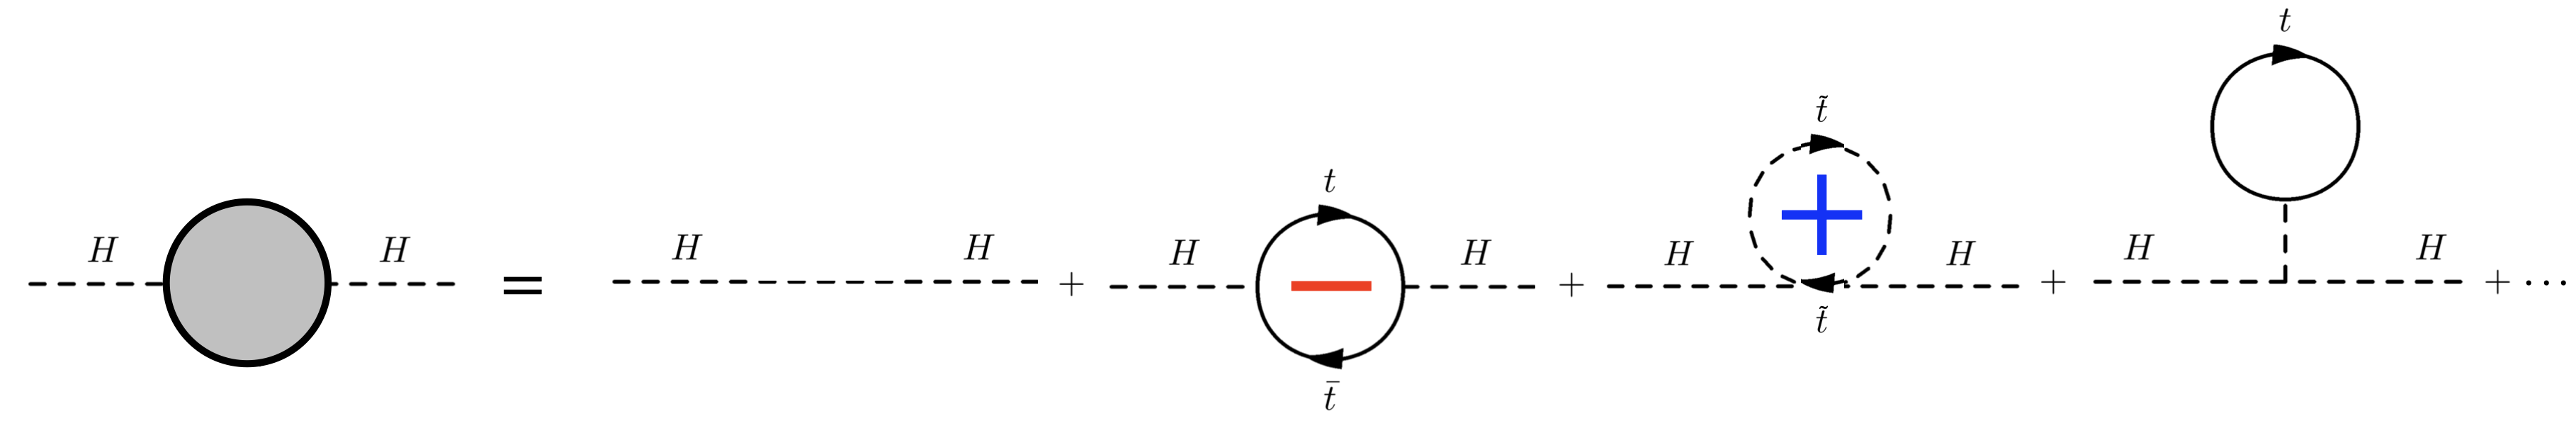
\includegraphics[width=0.98\textwidth]{figs/theory/HiigsMassLoopsSUSY.png}
  \end{center}
  \caption{The observed Higgs mass as a sum of the bare Higgs mass plus loop corrections now including contributions from SUSY particles. The large blue ``$\textcolor{blue}{+}$'' sign from the stop loop illustrating the it's effective cancellation with the top loop contribution with the red ``$\textcolor{red}{-}$'' sign.}
  \label{fig:theory:HiggsMassLoopsSUSY}
\end{figure}

\subsection{\emph{R}-parity}
%\textcolor{red}{\hrulefill \textsc{Unfinished Section}\hrulefill}\\
Within the framework of the MSSM it is now possible to construct terms in the Lagrangian that violate Baryon ($B$) and Lepton number ($L$) to the tune that the proton would decay in approximately $10^{-2}$ seconds (for $\mathcal{O}(1)$ \emph{R}-parity violating couplings, or if minimal flavor violation is assumed the lifetime can be extended to 1 year).
We know of course that the proton does not rapidly decay (with lifetime bounds currently at $6\times10^{39}$ years) and we also do not observe lepton number violation, so this problem must be addressed in the theory.
A popular solution is to add in a discrete symmetry known as ``\emph{R}-parity,'' defined as the following,
\begin{equation}
    \text{\emph{P}}_{R}=(-1)^{3(B-L)+2S} 
\end{equation}
Where $S$ is the spin of the particle.
When \emph{R}-parity is conserved at a vertex this forbids $B$ and $L$ violation entirely.
This seems like a pretty reasonable thing to do, as $B$ and $L$ seem to be pretty much conserved as far as we can tell.
Also this \emph{R}-parity conserving solution (RPC) necessarily demands that the Lightest Supersymmetric Particle (LSP) be stable\footnote{R=parity is also a measure for SUSYness, i.e. SUSY particles will always have $P_{R}=-1$ while SM particles will have $P_{R}=+1$}, which would give us a very convenient dark matter candidate.
While this discrete symmetry does indeed accomplish its purpose, \emph{R}-parity is, from a theoretical viewpoint, completely ad hoc, without any fundamental justification.




 

